\chapter{Literature Review} \label{chapter:literaturereview}
In this section we describe some techniques used in NLP, trying to give an overview of the current state of art and what is necessary to train a language model.

\section{Natural Language Processing}
\alert{Communication and the sharing of knowledge is an essential part of human society. History has shown that the best way to transmit knowledge is in writing. It is not difficult for a person to learn to read and to understand the context in texts. For computers, this task is much more difficult. Natural Language Processing (NLP) is a subfield pf Artificial Intelligence (AI) which deals with teaching computers to understand and interpret human language and has emerged in 1940. The initial need of NLP was the translation from one language into another which was used during the second world war. Nowadays it is widely used in health care, spam detection, sentiment and cognitive analysis. NLP also provides computers with the ability to read text, hear speech, and communicate with humans. Every person had contact with a NLP device at least once in their life. The best example everyone might know are personal assistants like Siri or Alexa. These are applications which work with NLP and have learned to communicate with humans and nearly seem humanely.\newline
Generally speaking, NLP breaks down language into shorter, more basic pieces, called tokens (words, periods, etc.) which get saved as vectorial representations. The technique of mapping words to real vectors is called word embedding. To understand the relationships of the tokens, the model gets trained by predicting some hidden part of the text using some other part of their surrounding text. One way to calculate the representations of the vectors is the method \textit{Word2Vec}. Until BERT has emerged, Word2Vec was the most common technique to create word embeddings. It is a two-layer neural network which processes text and turns it into a numerical form that can be understand by deep neural networks. Given enough data, Word2vec can make highly accurate guesses about a word’s meaning based on past appearances. Those guesses can be used to establish a word’s association with other words. The diference between Word2Vec and BERT will be covered in Section \ref{bert}}.

\section{Text Representation}
Text representation is a fundamental problem of NLP and necessary for preparing raw text as input for a language model. It aims to create a numerical representation of the unstructured text and make them mathematically computable. It is also called text vectorization or feature extraction.\newline
Texts cannot be processed by ML models directly. Tokenization is a method that transforms sequences of characters into a sequence of integers. As an example we can take the sentence: \newline

\centerline{"This is a cat."} 

A tokenization transforms this sentence into [‘This’, ‘is’, ‘a’, cat’]. Punctuations will be removed. This step is important to help the model understanding the meaning of a text. The model can
\begin{itemize}
	\item Count the number of words in the text
	\item Count the frequency of the word, that is, the number of times a particular word is present
\end{itemize} 

In modern LMs, tokenizers are trained together with the model to identify the best possible transformations, which can happen on both word and sub-word levels. The set of obtained tokens determines the vocabulary of an LM. If a word appears in the vocabulary of LM, it can be represented as a vector in the target space. Otherwise, a word is split into parts until each of them can be mapped to a set of tokens from the vocabulary. In the worst case, a word is split into individual letters. Such splitting may significantly reduce the quality of word embeddings in the vector space, thus reducing the quality of features extracted for the classification layers of a network. Therefore, it is essential either to select an LM whose vocabulary provides good coverage of the main terms used in an application domain or to extend the vocabulary of an LM with these terms and fine-tune it on domain-specific texts. 

The next chapters cover the most common techniques of text representation.

\subsection{One-Hot Encoding}
One-hot encoding is a type of representation which sentences in a document into the shape of a 2-D array as shown in the example below for the sentence \textbf{This is a cat.}:

\begin{table}[H]
	\centering
	\begin{tabular}{ll}
		\hline
		\textbf{Word} & \textbf{Vector Representation} \\ \hline
		This & [1, 0, 0, 0]\\ 
		is    & [0, 1, 0, 0]\\ 
		a & [0, 0, 1, 0]\\ 
		cat  & [0, 0, 0, 1]\\ \hline
	\end{tabular}
	\caption{One Hot Encoding Example}
	\label{tab:onehot}
\end{table}

\subsection{Term Frequency - Inverse Document Frequency}
Term Frequency - Inverse Document Frequency (TF-IDF) is a statistical measure to determine how important a word is within a document. It determines not only how often a word appears in a single document, but also how often it appears in the entire document corpus. Very common words like "this" or "and" get a lower score, even though they occur often, because they are not important for the context of a document. This will be determined by comparing the occurrence of these words among the documents. This strategy is often used in NLP for text analysis. For example, in a failure analysis report, a word like failure would get a high score. By using other important words, the report could be automatically assigned to a certain failure type and thus classified. \\
TF-IDF for a word in a document is calculated by multiplying the term frequency and the inverse document frequency.

\begin{align}
	tf idf (t, d, D) &= tf(t, d) * idf(t, D)
\end{align}
Where
\begin{align}
	tf (t, D) &= log(1 + freq(t, d)) \\
	idf(t, D) = log(N/count(d E D, t E d))
\end{align}

The term frequency \textit{tf} is either a simple count of instances a word appears in a document or it can be adjusted by taking the length of the document to account. The calculation can be seen in (2.3) where \textit{t} is the term and \textit{D} the document to analyse. The inverse document frequency \textit{idf} is determined accross the document corpus. The closer this metric is to zero, the more common a word is. The calculations can be seen in (2.4) where \textit{N} is the number of documents.

\subsection{Bag of Words}
Bag of Words is a method for simplifying the representation of documents and the importance of the words they contain which is used in NLP and Information Retreivel (IR). Here the sentences in the documents are divided into their individual words and counted. The resulting object contains a list of the contained words and the number of their occurrences. It is called a “bag” of words, because any information about the order or structure of words in the document is discarded. The model is only concerned with whether known words occur in the document, not where in the document. We will describe the concept of bag-of-words with the following example: The below snippet contains the first few lines of \alert{the book "A Tale of Two Cities" by Charles Dickens. Different example?}


\textit{
\centering	
It was the best of times,\\
it was the worst of times,\\
it was the age of wisdom,\\
it was the age of foolishness, \\
}

In this example, each line will be treated as an individual document. The model vocabulary is containing the following 10 words:
\begin{itemize}
	\item “it”
	\item “was”
	\item “the”
	\item “best”
	\item “of”
	\item “times”
	\item “worst”
	\item “age”
	\item “wisdom”
	\item “foolishness”
\end{itemize}

Using this vocabulary, vector representations can be created for any document. For this purpose, a suitable scoring method must be chosen. The scoring method can be binary scoring or frequencies. Table \ref{tab:scoring} is showing an example of the resulting vector representations for a document which contains the first line in our example.

\begin{table}[H]
	\centering
	\begin{tabular}{ll}
		\hline
		\textbf{Scoring Method} & \textbf{Resulting Vector Representation}                                         \\ \hline
		Binary & [1, 1, 1, 1, 1, 1, 0, 0, 0, 0] \\ \hline
		Frequencies & [1, 1, 1, 1, 1, 1, 0, 0, 0, 0] \\ \hline
	\end{tabular}
	\caption{Example of scoring methods}
	\label{tab:scoring}
\end{table}



\subsection{Word Embeddings}
A machine is not able to process text in its raw form. Word embedding is a technique were words are transformed into a numerical representation, a vector. This embedding is then fed into machine learning models. The simplest embedding technique is one hot encoding which would look as in Table \ref{tab:onehot}.

\begin{table}[H]
	\centering
	\begin{tabular}{ll}
		\hline
		\textbf{Word} & \textbf{Vector Representation} \\ \hline
		have & [1, 0, 0, 0, 0, 0, ... 0]\\ 
		a    & [0, 1, 0, 0, 0, 0, ... 0]\\ 
		good & [0, 0, 1, 0, 0, 0, ... 0]\\ 
		day  & [0, 0, 0, 1, 0, 0, ... 0]\\ \hline
	\end{tabular}
	\caption{One Hot Encoding Example}
	\label{tab:onehot}
\end{table}

Because the vector representations may get quite large with one hot encoding, there is the need of more effective encoding techniques.

\subsubsection{Word2Vec Architecture}
Word2vec is not a singular algorithm, it is a family of model architectures and optimizations that can be used to learn word embeddings from large datasets. The strength of Word2Vec lies in assigning similar vectors to words with similar meanings. 






\section{Masked Language Modelling}

\subsection{Transformer}
The transformer in the field of NLP is a new architecture which is able to solve sequence-to-sequence tasks while handling dependencies in the text. Transformers basically consist of an encoder and a decoder. The encoder reads the input text and the decoder produces a prediction. Transformers work in small increments. In each step, an attention mechanism is applied to understand the relationships between the words in a sentence, regardless of their positions. Both encoder and decoder sections of transformer are a stack of 6 identical layers of multi-head attention and feed forward sublayers. \alert{Each sublayer takes a residual connection from its previous inputs, adds it to the sub layer output and normalises it to produce final output of the sub layer. To allow for residual addition, all sub-layers produce an output of dimension 512.} The architecture is depicted in Figure \ref{fig:transformer}.


\begin{figure}[H]
	\centering
	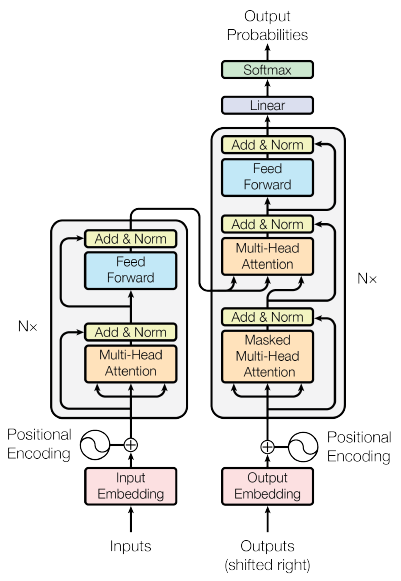
\includegraphics[width=0.5\textwidth]{figures/transformer_architecture.png}
	\caption{Transformer Architecture}
	\label{fig:transformer}
\end{figure}

\subsection{Evolution of Language Models}
It has always been difficult to teach a computer to really understand natural language. While they are capable of processing and storing large amounts of data, they lack language context. This problem continued until NLP became popular in the Artificial Intelligence field. NLP enables computers to read, analyze, interpret and gather information from long texts and single written words. In contrast to before without NLP, meaning and sense of texts can now be determined. In the beginning, a separate model was developed and used for each of these tasks. Since the development of BERT in 2018, this has changed. Engineers are now able to use a single model to handle the most common NLP tasks such as Classification, Sentiment Analysis or Question Answering. The timeline depicted in Figure \ref{fig:timeline} shows the evolution of NLP models from \alert{Bag OF Words} until \alert{BERT}.

\begin{figure}[H]
	\centering
	\includegraphics[width=1\textwidth]{figures/timeline_NLP.PNG}
	\caption{Timeline of Model evolution in NLP.}
	\label{fig:timeline}
\end{figure}

The following sections will briefly describe all of the mentioned models to cover all the important topics which will be discussed in this paper and to prepare for the technical details of BERT.

\subsection{BERT} \label{bert}
BERT  stands  for  Bidirectional Encoder Representations from Transformers. It makes use of a transformer and an attention mechanism that learns contextual relations between words or sub-words in a text. The BERT model was developed by Google researchers in 2018 and is already pre-trained using a combination of masked language modeling objective and next sentence prediction on a large corpus. The original BERT model comes in two sizes: BERT-base (trained on BooksCorpus: ~800 million words) and BERT-large (trained on English Wikipedia: ~ 2,500 million words). 
In contrast to previous language models which looked at a text sequence either from left to right or combined left-to-right and right-to-left training, BERT is using the bidirectional approach. The paper’s results show that a language model which is bidirectionally trained can have a deeper sense of language context and flow than single-direction language models. To do this, the authors introduced a new technique which is called Masked Language Modelling (MLM). \alert{This objective randomly masks 15\% tokens from an input sequence and trains on the model to predict the original vocabulary id of the masked word based on it context. This approach allows the representations to fuse context from either ends. Rather than always masking the chosen word, it masks the word 80\% times with [MASK] token, 10\% times with any random word and remaining 10\% times with the actual word, thereby biasing the prediction towards the actual observed word. Another pre-training feature introduced in BERT is ‘Next Sentence Prediction’ that takes in a sentence-pair input, replaces the second input sentence with a random sentence for 50\% of the training steps, and trains on the sentence pairs to learn sentence relationships which is needed for many downstream tasks like Question Answering and Natural Language Inference.} \newline
A Transformer usually includes two separate mechanisms, an encoder that reads the text input and a decoder that produces a prediction for the task. For producing a language model, only the encoder mechanism is necessary. Previous models have read the text input sequentially either left-to-right or right-to-left. BERT's transformer encoder reads the entire sequence of words at once. This allows the model to learn the context of a word based on all of its surroundings\alert{ \cite{Devlin}}.  \newline
The input to BERT's encoder is a sequence of tokens previously converted into vectors. Later, these tokens can be processed in the neural network. In order to be able to do this, a few steps must first be carried out:
\begin{enumerate}
	\item CLS and SEP tokens at the beginning and end of each sentence
	\item Segment embeddings for each token to distinguish between sentences.
	\item Position embeddings for each token to identify the position in a sentence.
\end{enumerate}
These three steps are depicted in Figure \ref{fig:bert_tokenizing}.

\begin{figure}[H]
	\centering
	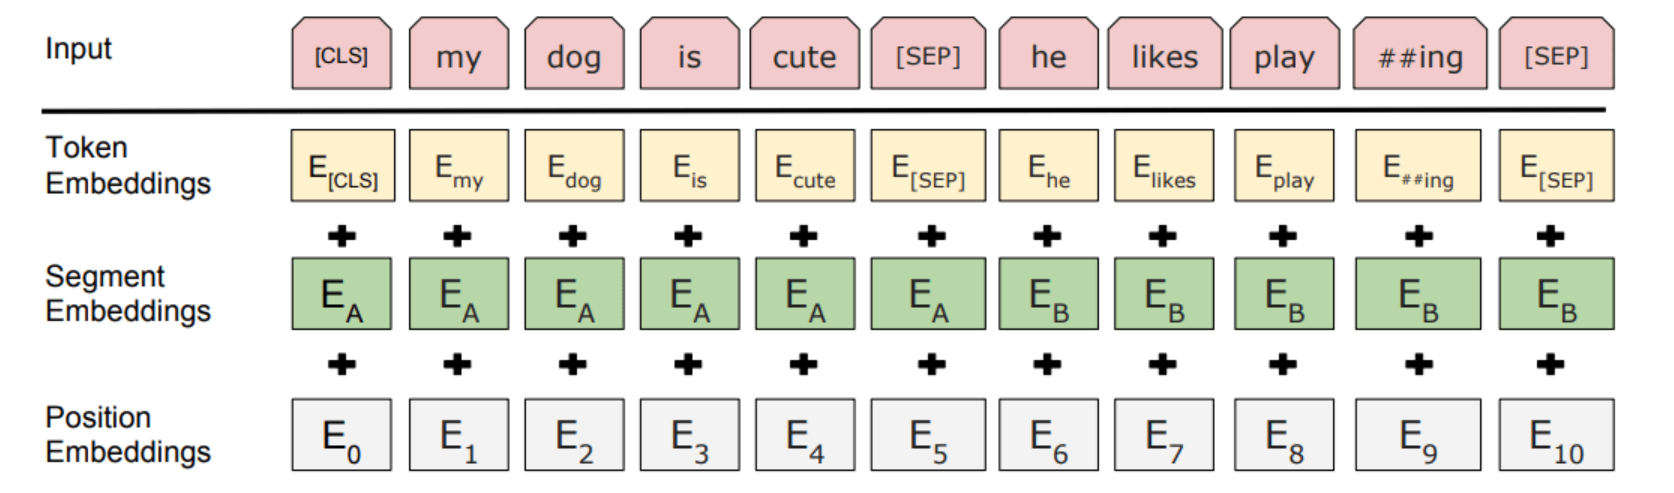
\includegraphics[width=1\textwidth]{figures/bert_tokenizing.png}
	\caption{Embeddings of Text Input with BERT.}
	\label{fig:bert_tokenizing}
\end{figure}

\begin{figure}[H]
	\centering
	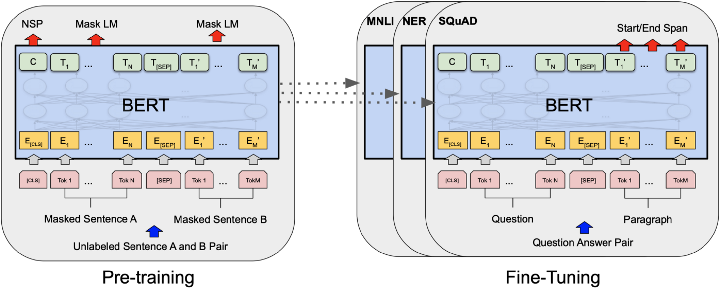
\includegraphics[width=1\textwidth]{figures/bert_training.png}
	\caption{Pre-Training and Fine-Tuning Process of BERT}
	\label{fig:bert_tokenizing}
\end{figure}

\subsubsection{Difference from BERT and word2Vec}
Word2Vec is contex-independent, so it only has a numeric vector to represent a word. If a word has several meanings, these are combined into a vector.

BERT, on the other hand, is context-dependent and thus allows multiple numeric vectors as a representation for a word, depending on the context in which the word occurs.

An example of the difference is the word bank, which can appear in a financial context as well as in a beach or park context. Word2Vec will always generate the same vector for this word and can therefore lead to an inaccurate representation. BERT can distinguish the two different semantic meanings and thus also generate two different vectors.

\begin{enumerate}
	\item The next difference is that Word2Vec doesn't care about the position of words in a sentence. BERT, on the other hand, uses the position (index) of a word as input for calculating the vector.
	\item Word2Vec only needs one word as input and delivers a vector as output. BERT, on the other hand, needs an entire sentence as input because it needs the context of the sentence to calculate the vector.
	\item Word2Vec can have problems if a word is not stored in the vocabulary and no vector can be generated. BERT can also create a vector for subwords that are not stored in the vocabulary and is therefore not limited by the vocabulary.
\end{enumerate}

